 \documentclass[10pt,oneside,swedish]{lips-no_customer}

%\usepackage[square]{natbib}\bibliographystyle{plainnat}\setcitestyle{numbers}
\usepackage[round]{natbib}\bibliographystyle{plainnat}
\usepackage{parskip}
\usepackage{subfigure}
\usetikzlibrary{decorations.pathreplacing,angles,quotes}

\usepackage{pgfplots}
\usepackage{pgfplotstable}

% Configure the document
\title{Teknisk dokumentation}
\author{Yc4}
\date{\today}
\version{0.4}

\reviewed{}{}
\approved{}{}

\projecttitle{Styrning och optimering av bilbana}

\groupname{Yc4}
\groupemail{team\_yc4@liuonline.onmicrosoft.com}
\groupwww{https://www.fs.isy.liu.se/Edu/Courses/TFYY51/}

\coursecode{TFYY51}
\coursename{Ingenjörsprojekt}

\orderer{Erik Frisk, Linköpings universitet}
\ordererphone{+46(0)13-285714}
\ordereremail{erik.frisk@liu.se}

%\customer{Kund, Företag X}
%\customerphone{+46 xxxxxx}
%\customeremail{erik.frisk@liu.se}

\courseresponsible{Urban Forsberg}
\courseresponsiblephone{+46(0)13-281350}
\courseresponsibleemail{urban.forsberg@liu.se}

\supervisor{Viktor Leek}
\supervisorphone{+46(0)13-284493}
\supervisoremail{viktor.leek@liu.se}

\smalllogo{logo} % Page header logo, filename
\biglogo{logo} % Front page logo, filename

\cfoot{\thepage}
\begin{document}
\maketitle

\cleardoublepage
\makeprojectid

\begin{center}
  \Large Projektdeltagare
\end{center}
\begin{center}
  \begin{tabular}{|l|l|l|}
    \hline
			\textbf{Namn} & \textbf{Ansvar} & \textbf{Kontaktinformation}\\
		\hline
			Mattias Uvesten & Projektledare (PL) & 0768697559\\
			&& \url{matvu053@student.liu.se} \\
    \hline
			Gustav Sörnäs & Dokument, display (DOK, DSP) & 0703279113\\
			&& \url{gusso230@student.liu.se} \\
    \hline
			Alexander Tuneskog & Hastighet (SPD) & 0725559873 \\
			&& \url{aletu130@student.liu.se} \\
    \hline
			David Thorén & Tester, gemensam målgång (TST, GML) & 0721838605 \\
			&& \url{davth346@student.liu.se} \\
    \hline
			Albin Wahlén & Kalibrering, positionering (KLB, POS) & 0762016054 \\
			&& \url{albwa833@student.liu.se} \\
    \hline
  \end{tabular}
\end{center}

\section*{Dokumenthistorik}
\begin{tabular}{p{.06\textwidth}|p{.1\textwidth}|p{.45\textwidth}|p{.13\textwidth}|p{.13\textwidth}} 
  \multicolumn{1}{c}{\bfseries Version} & 
  \multicolumn{1}{|c}{\bfseries Datum} & 
  \multicolumn{1}{|c}{\bfseries Utförda förändringar} & 
  \multicolumn{1}{|c}{\bfseries Utförda av} & 
  \multicolumn{1}{|c}{\bfseries Granskad}\\
  \hline
		0.1 & 2019-11-28 & Struktur & Alla \\
  \hline
		0.2 & 2019-11-30 & Första utkast & Alla & \\
  \hline
		0.3 & 2019-12-01 & Andra utkast & Alla & \\
  \hline
 		0.4 & 2019-12-02 & Tredje utkast & Alla & \\
  \hline
  
\end{tabular}

\cleardoublepage
\pagenumbering{arabic}\cfoot{\thepage}
% \section*{Sammanfattning}
Massa text som sammanfattar hela skiten.



\cleardoublepage
\tableofcontents
\cleardoublepage

\section{Inledning}
Projektet ska utveckla ett system vilket styr bilar runt en bilbana efter en given referenstid. Till förfogande finns, en bilbana, ett antal bilar, en display samt en dator.
Målet med detta projekt är att bilarna skas köras runt banan inom 0,5 sekunder av den referenstid som användaren har angett. Efter en avslutad
körning på x varv ska standardaviklesen på varvtiderna inte överskrida 0,2 sekunder. Systemet skrivs i MatLab och har som huvudsyfte att reglera den spänning som bilbanan skickar
till bilarna. Olika bilar beter sig olika utifrån vissa skillnader bland bilarna, till exempel vikt, motorn i dem samt den magnet under bilarna som håller dem någorlunda fast på banan. 
Hela systemet ska styras utifrån en touch display som är enkel att förstå för gemene man och efter avslutad körning ska den även visa statistik om hur körningen gick. 
\begin{figure}
	\centering
	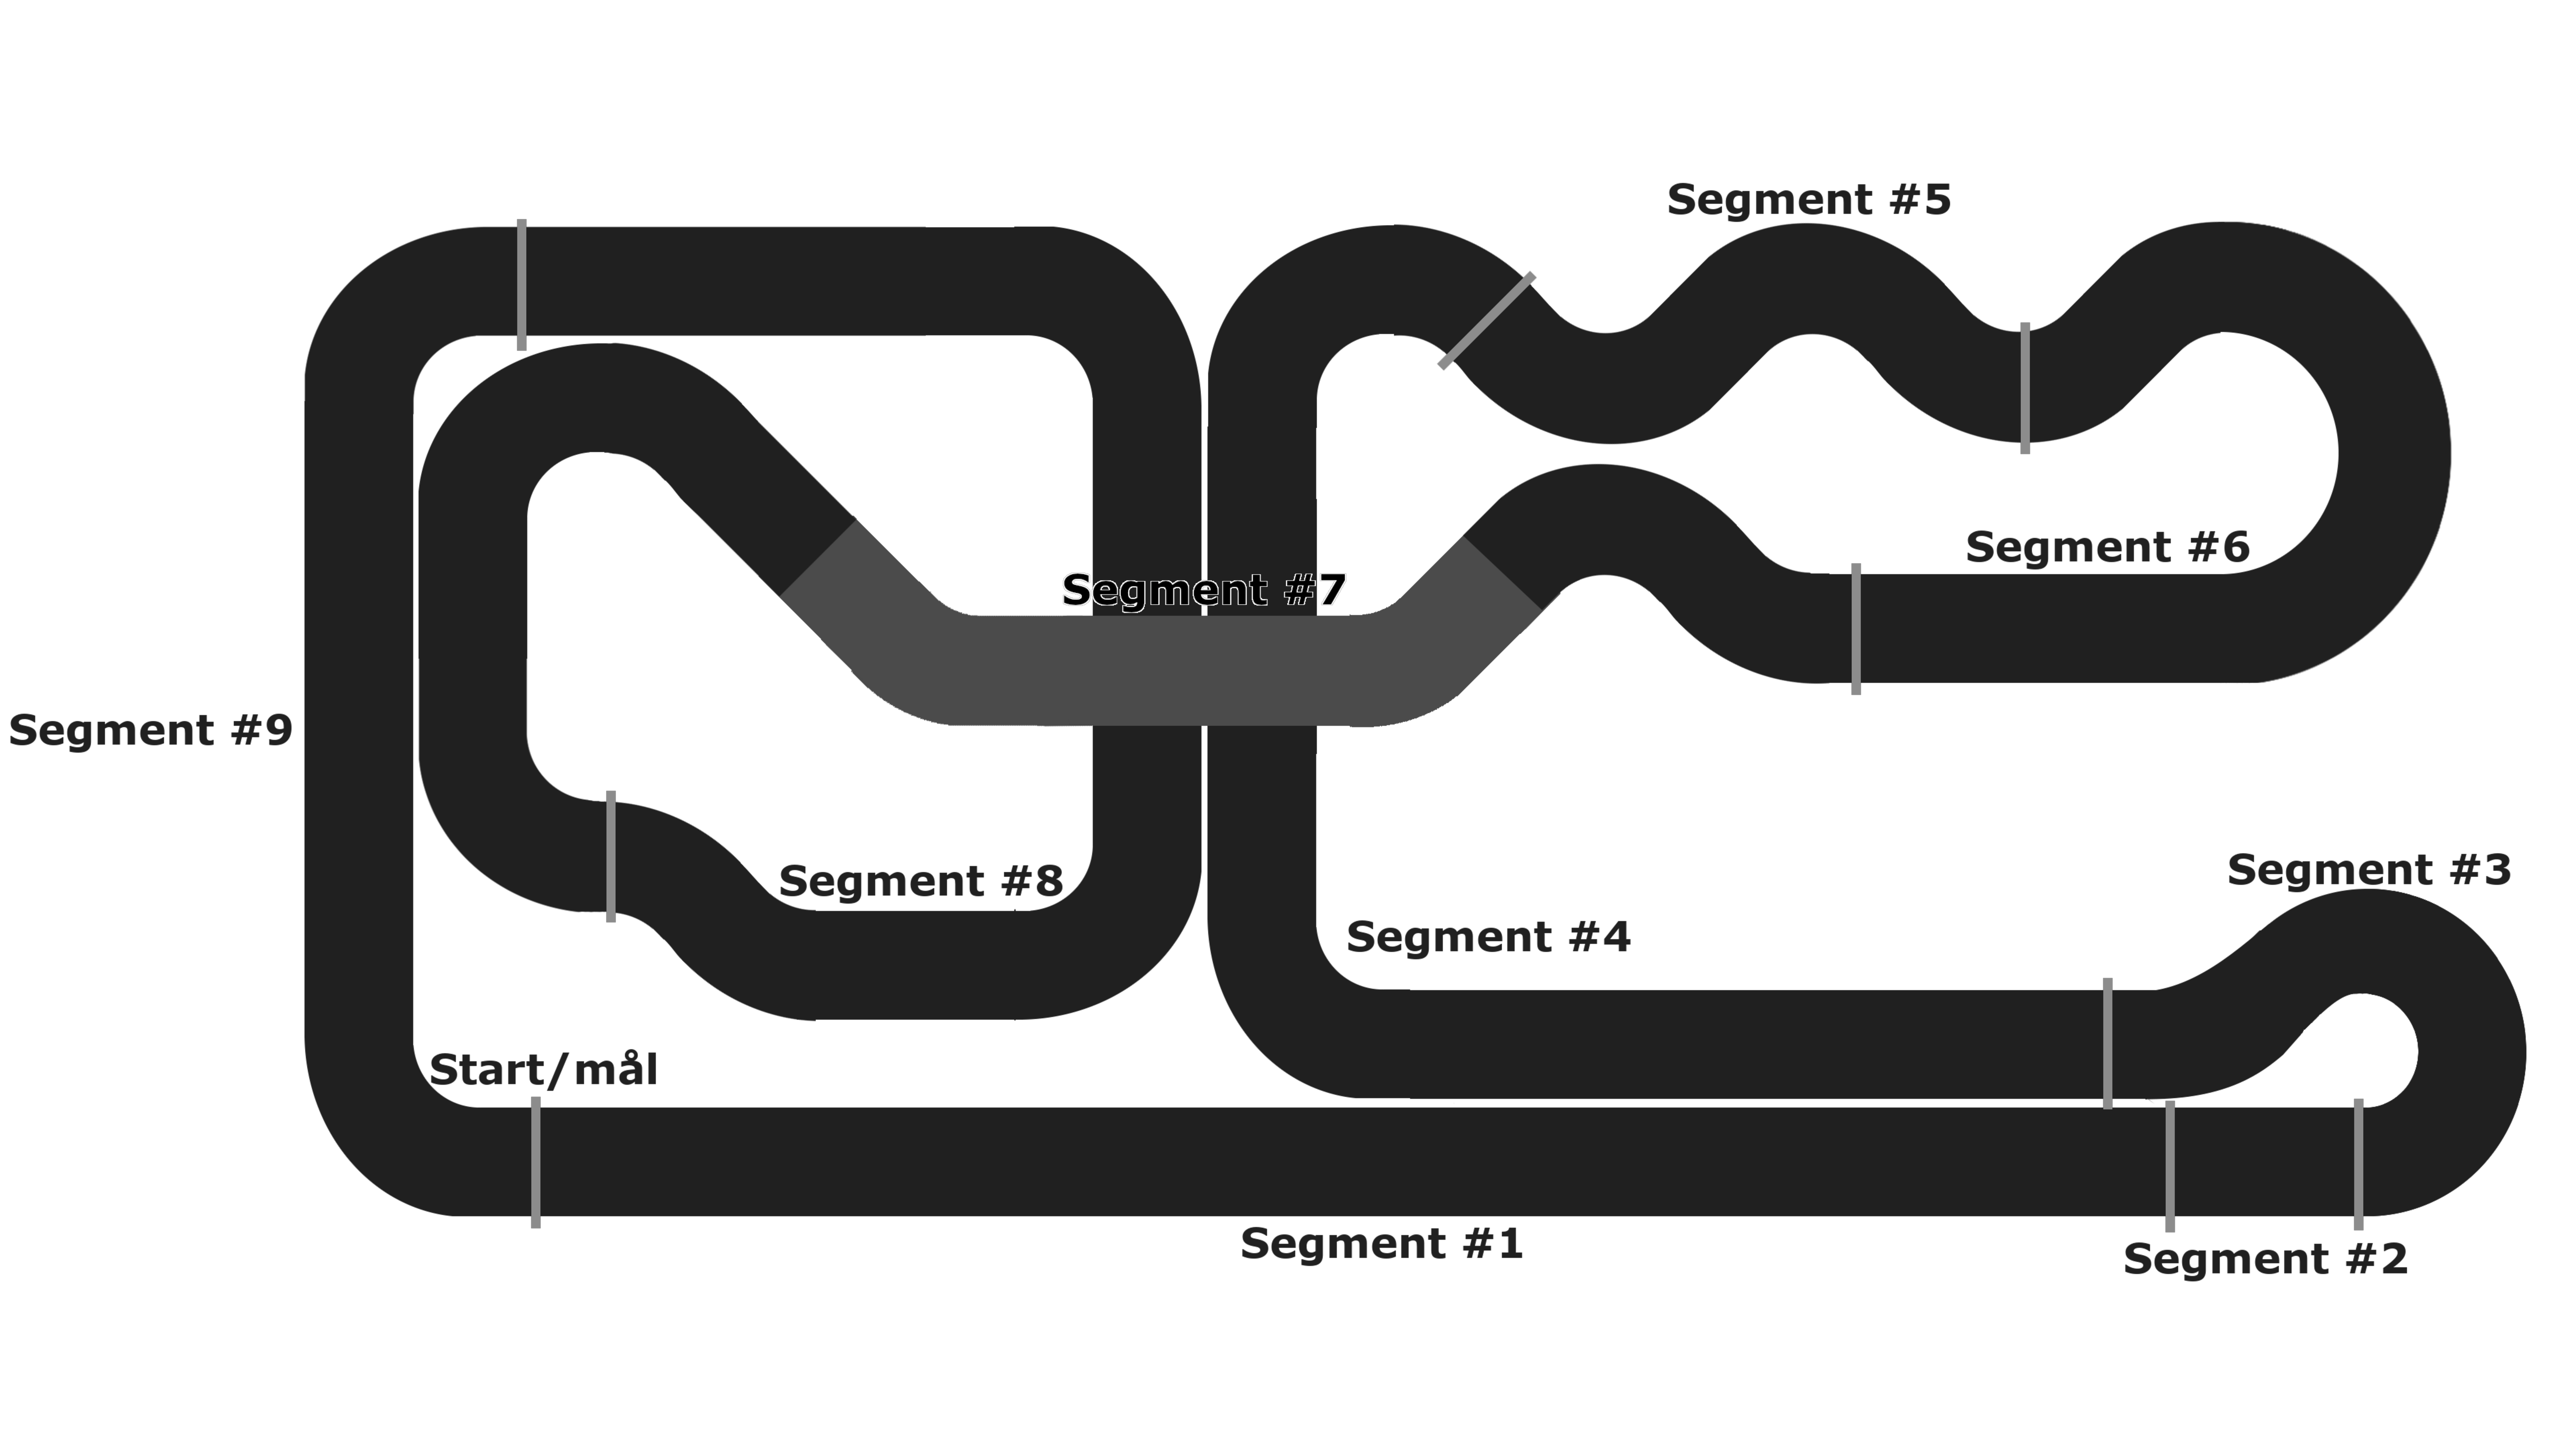
\includegraphics[width=\linewidth] {Figures/BanaModell}
	\caption{En modell av bilbanan.}
	\label{fig:bilbanan}
\end{figure}

\subsection{Bakgrund} 

Projektet har utförts med hjälp av en bilbana samt flera bilar, givare,
spänningsaggregat och två datorer inne i bilbanerummet. Via datorn har spänning
tillförts till bilbanan. Med hjälp av givarna är det möjligt att veta när en bil
har passerat en givare. Programvaran har utvecklats i Matlab.

\subsection{Syfte och mål}

Syftet med projektet är att lära sig att arbeta i ett projekt utifrån
projektstyrningsmodellen LIPS. Målet med projektet var att konstruera ett system
som kunde köra bilar runt en bilbana på en vald referenstid mellan 12 och 15
sekunder. Detta skulle göras för flera bilar med olika egenskaper. Fler krav som
ska klaras av finns i kravspecifikationen (\ref{app:kravbeskrivning}).

\subsection{Avgränsningar}

- Ingen gemensam målgång

\section{Begrepp och systemöversikt}
\label{sec:begrepp och systemöversikt}

Runt om bilbanan finns nio givare som skickar en signal när en bil passerar under
dem. En av givarna kallas målgivaren vars signal går att skilja från övriga
givare och således passar som en markör när ett nytt varv inleds. Givarna
delar in banan i nio delar, kallade segment. Dessa segment har i sin tur delats
in i totalt 80 delsegment där ett delsegment motsvarar en fysisk bit av banan.
För vardera bana och delsegment har ett värde på en \emph{spänningsparameter}
tagits fram. Detta värde varierar dels eftersom bilarna vid olika delar av banan
behöver olika mycket spänningstillförsel för samma hastighet och dels eftersom
bilarna vid vissa delar av banan inte kan åka lika snabbt som vid andra delar av
banan för att inte riskera att åka av. En spänningsparameter är i det här fallet
ett värde som i slutändan kommer multipliceras med en parameter för bilen för
att ge en slutlig signal att skicka till banan.

Centralt för systemet är den karta som beskrivs ovan samt en
modifierare som beror på köregenskaperna för den nuvarande bilen. Det
modifierande värdet kallas bilens \emph{konstant}. Denna konstant varierar
beroende på hur mycket spänning en viss bil behöver för att nå en viss
hastighet. Konstanten anpassas under körningens gång ytterligare beroende på
bilens varvtid jämfört med referenstiden.

\subsection{Display}

Förrutom bilbanan finns även en \emph{display}. Innan körningen används denna för att välja vilka banor som ska köras, om de ska köras manuelt eller autonomt och vilken referenstid som ska köras mot. Under körningen visas i realtid det gaspådrag som skickas till banan. Efter körningen visas statistik i form av varvtider och den genomsnittliga tiden per segment.

\subsection{Kommunikation}

För att rita object på displayen finns hjälpfunktioner liknande ett API som
tagits fram utifrån displayens tekniska specifikation, se bilaga displayspecifikation.
Hjälpfunktionerna implementerades i Matlab och beskrivs i sin helhet i Appendix
del~\ref{app:funktioner och filer:display}.

För att reagera på knapptryck på displayen kan displayen instrueras att flytta
hela sitt interna minne (där information om bland annat knapptryck finns) till
ett minne som delas med styrdatorn. Detta minne kan sedan läsas av och systemet
kan agera utifrån händelserna som har skett.

% \begin{itemize}
% 
% 	\item \texttt{car.num} - Om bilen är på bana ett eller två.
% 	\item \texttt{car.running} - Om bilen körs eller inte.
% 	\item \texttt{car.stopping} - Om bilen för tillfället letar efter ett ställe att stanna på.
% 	\item \texttt{car.stopped} - Om bilen har hittat ett ställe att stanna på.
% 	\item \texttt{car.automatic} - Om bilen ska köras autonomt.
% 	\item \texttt{car.segment} - Bilens nuvarande segment.
% 	\item \texttt{car.lap} - Bilens nuvarande varv.
% 	\item \texttt{car.lap\_times} - En lista över bilens varvtider.
% 	\item \texttt{car.seg\_times} - En matris över bilens segmentstider per varv.
% 	\item \texttt{car.position} - Bilens position i meter efter målgivaren.
% 	\item \texttt{car.pos\_at} - En lista över hur långt det är kvar till målgivaren från de olika segmenten.
% 	\item \texttt{car.seg\_len} - En lista över längden för varje segment.
% 	\item \texttt{car.percents} - En lista över hur stor andel av varvtiden varje segment förväntas ta.
% 	\item \texttt{car.map} - Kartan över alla subsegment och önskad spänningstillförsel.
% 	\item \texttt{car.miss\_probability} - Sannolikheten att bilen vid en given givare inte får en signal. Används för att testa krav 3.
% 	\item \texttt{car.constant} - Multipliceras med den önskade spänningstillförseln för att
% 		kompensera för olika bilars olika påverkan av samma spänningstillförsel.
% 
% \end{itemize}
% 
% 
% Utöver dessa värden sparas ett antal värden för själva systemet.
% 
% \begin{itemize}
% 
% 	\item \texttt{display.data} - En kö av kommandon som ska skickas till displayen.
% 	\item \texttt{bootN.status} - Om den så kallade ''bootstrapen'' är aktiv för bana N. Se \ref{sec:systembeskrivning:uppstart}
% 	\item \texttt{bootN.time} - Den tid som passerat sedan förra gången ''bootstrapen'' höjde \texttt{car.constant} för bana N. Se 
% 	\ref{sec:systembeskrivning:uppstart}
% 	\item \texttt{halt} - Om någon av bilarna åkt av och användaren valt att avbryta körningen.
% 	\item \texttt{t} - Hur lång tid den nuvarande programcykeln tagit.
% 	\item \texttt{highToc} - Längden på den längsta programcykeln. Används för att kontrollera krav 31.
% 
% \end{itemize}

\section{Systembeskrivning}

% Systemet funktion vid starten är att öka oftare i början bootstrapen
% (exempelvis innan målgivaren) för att sedan öka mindre frekvent i segment 1.
% Bootsrapen (uppstarten) avslutas efter segment 3. 

\begin{figure}
	\centering
	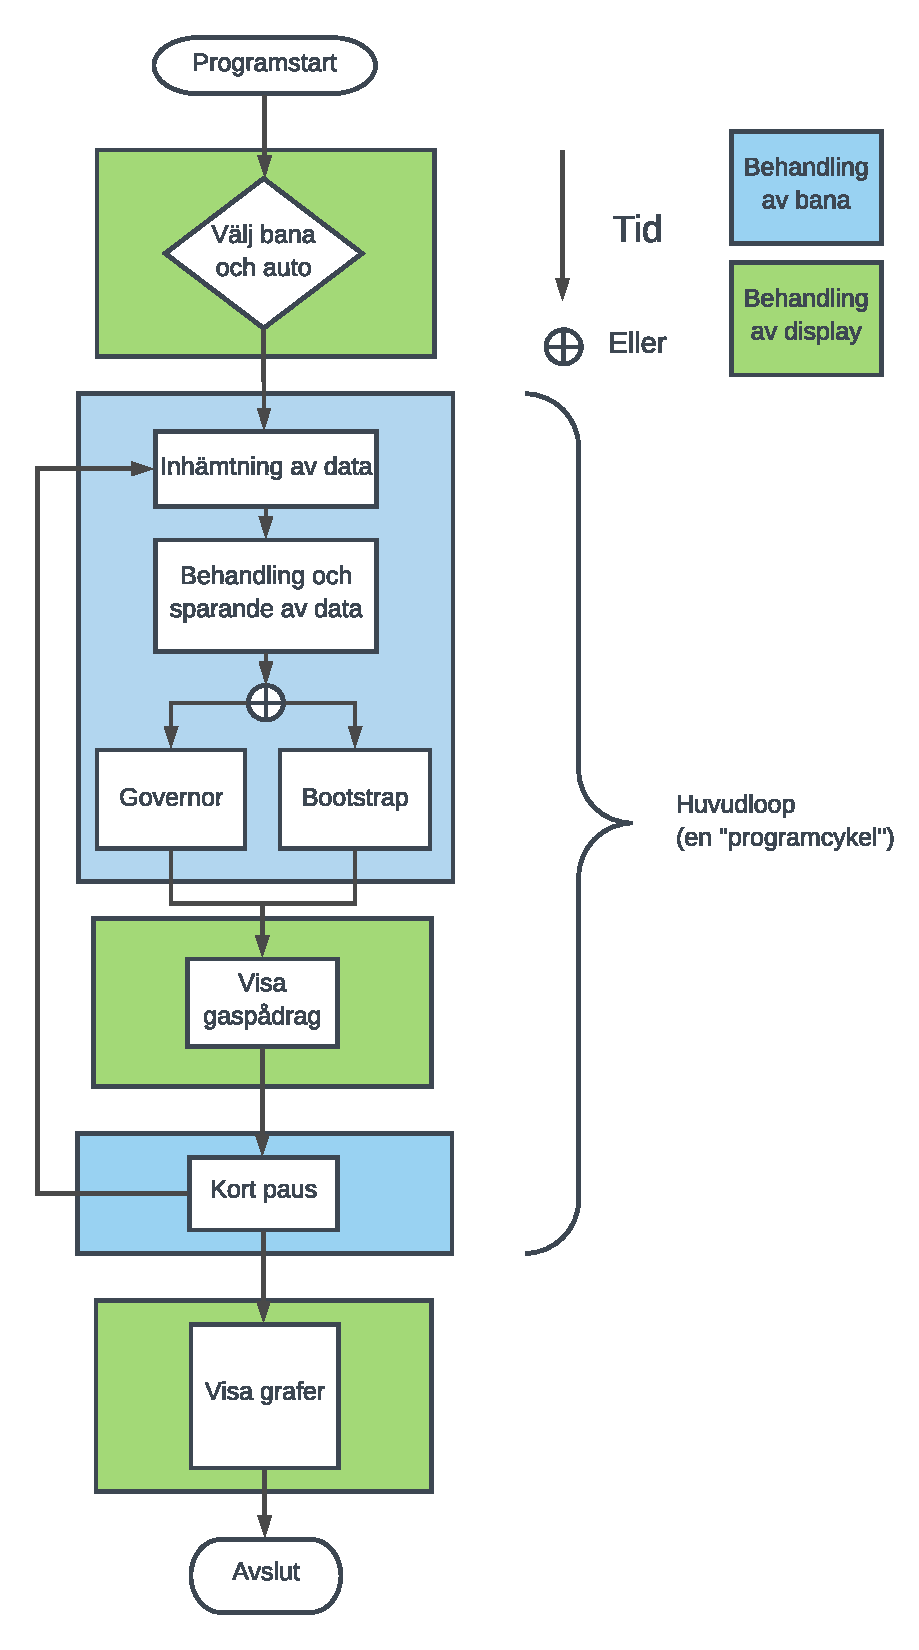
\includegraphics [height=0.8\textheight] {Figures/flow}
	\caption{Flödesschema över systemet.}
	\label{fig:flow}
\end{figure}

Systemet är indelat i olika delsystem efter huvudsaklig funktionalitet enligt figur
\ref{fig:flow}. Nedan beskrivs dessa delsystem i mer detalj.

\subsection{Innan start}

Vid uppstart ritas knappar ut på displayen, se figur x. Med dessa knappar går
det att välja om en eller två banor ska vara aktiva och om de ska styras
autonomt av systemet eller manuellt med handkontroll. Det går också att ställa
in en referenstid mellan 12 och 15 sekunder med 0,5 sekunders intervall genom
att trycka på + och - på displayen. 

\subsection{Uppstart} 
\label{sec:systembeskrivning:uppstart}
Vid autonom körning utgår systemet ifrån en bootstrap som är till för uppstarten av bilarna. Då körs funktionen \texttt{do\_boot()} som arbetar fram en
initial \texttt{car.constant}. Detta sker i tre steg. Innan bilen börjar rulla
höjs \texttt{car.constant} varje 0,7 sekunder. När bilen börjar rulla och åker
under målgivaren höjs \texttt{car.constant} långsammare tills bilen åkt under
den första givaren varpå \texttt{car.constant} inte längre ändras. Vid den
tredje givaren jämförs hur lång tid det senaste segmentet tog att köra och en
sista \texttt{car.constant} räknas ut som förväntas ge en varvtid på 15
sekunder. Om den förväntade varvtiden är längre än 15 sekunder höjs
\texttt{car.constant} och om den förväntade varvtiden är lägre sänks
\texttt{car.constant}.

\subsection{Körning}
\label{sec:systembeskrivning:korning}

Körningen är uppdelad i olika faser. Dessa presenteras nedan. En
\emph{programcykel} är när dessa faser körs igenom en gång. Samlingsnamnet för
faserna är \emph{huvudloopen}. Systemet behöver köra programcykler med som högst
0,1~sekunders intervall (enligt krav 31). I en programcykel beräknar systemet
var bilen befinner sig, hur snabbt bilen ska köra och skickar det nya
gaspådraget till banan. När en givare passeras justeras också bilens konstant
efter nuvarande varv- och referenstid.  Nedan beskrivs vad systemet gör under en
komplett programcykel.

\subsubsection{Position}
\label{sec:system:korning:position}

Om en givare passerats vet systemet exakt var bilen befinner sig. Om så är
fallet sparas den nuvarande exakta position och kallas \emph{givarpositionen}.

% Om en ny givare har passerats, \texttt{car.new\_check\_point == true}, ökar
% programmet nuvarande segment (\texttt{car.segment}) med 1. \texttt{car.segment}, som
% alltid ligger mellan 1 och 9, används som index för att välja position i en
% lista (\texttt{car.pos\_at}). Vi kallar den positionen för \emph{givarpositionen}.

Oavsett om en givare passerats eller inte räknar systemet ut en beräknad
position. Detta görs genom att räkna ut en approximativ hastighet $v =
\frac{s}{t}$ där $v$ är hastigheten, $s$ är längden på det nuvarande segmentet
och $t$ är hur lång tid det nuvarande segmentet tog förra varvet.

% Om ingen givare har passerars och första varvet är avslutat kallas först på
% funktionen \texttt{get\_approx\_v()}. Denna utgår ifrån förra varvets
% segmentstider (\texttt{car.seg\_times}) och segmentslängder
% (\texttt{car.seg\_len}) och beräknar med $v = \frac{s}{t}$, där \texttt{s} är
% segmentslängden och \texttt{t} segmentstiden, \texttt{v} som är
% medelhastigheten för nuvarnade segment, men förra varvet. Denna antas vara
% ungefär samma som nuvarande hastiget och kallas \emph{car.v}. 

Med den approximativa hastigheten räknar sedan systemet ut hur långt bilen rört
sig sen den senaste programcykeln. Denna förflyttning räknas ut med $\mathrm{d}s
= v \cdot \mathrm{d}t$ där $\mathrm{d}s$ är den beräknade förflyttningen, $v$
hastigheten som precis räknades ut och $\mathrm{d}t$ tiden sedan den förra
programcykeln. Denna förflyttning läggs till positionen från förra programcykeln
och kallas den \emph{beräknade} positionen.

Om en givare passerats upskattar systemet sedan om en givare vid ett tidigare
tillfälle passerats (genom att jämföra givarpositionen och den beräknade
positionen). Information om denna procedur finns i del~\ref{sec:missade givare}.

% Sedan beräknas positionen, i meter från målgivaren, med funktionen
% \texttt{get\_position()}. Den använder den ungefärliga hastigheten \texttt{v} beräknad av
% \texttt{approx\_v()} och tiden \texttt{t} sedan denna beräkning gjordes senast (en programcykel, se \ref{sec:system:korning:cykel})
% och beräknar med $s = v \cdot t$ den sträcka som bilen har åkt. Sedan adderas denna
% med förra kända positionen och returneras i \texttt{car.position}. Denna 
% \emph{beräknade} position tas också fram när en givare har passerats, då skrivs den över med \emph{givarpositionen} men används i stället för att detektera missade givare. Se \ref{sec:missade givare}.

\subsubsection{Gaspådrag}

Efter positionsberäkningen beräknas spänningen som ska skickas till banan. Först används positionen för att välja en spänningsparameter. Denna finns i kartan som är indexerad efter position. Gaspådraget ($u$) fås sedan genom att multiplicera denna hastighetsparameter ($v$) med bilens konstant ($k$): $u = v \cdot k$.

% Efter positionsberäkningen beräknas det gaspådrag som skall sättas till banan. Detta görs i två
% funktioner, \texttt{get\_new\_v} och \texttt{get\_new\_u}.
% 
% I \texttt{get\_new\_v} används bilens nuvarande postition (\texttt{car.postition})
% och hastighetskartan (\texttt{car.map}). I \texttt{car.map} finns en
% hastighetsparameter för varje \texttt{car.position} (Se \ref{sec:begrepp och systemöversikt}.), denna retuneras av funktionen
% och sparas i \texttt{car.v}.
%  
% I \texttt{get\_new\_u} används denna hastighetsparameter tillsammans med
% \texttt{car.constant}. Dessa multipliceras och deras produkt retuneras och sparas
% i \texttt{car.u}.

\subsubsection{Governor}
\label{sec:systembeskrivning:governor}

Om bootstrap är avslutad och en givare passerats behöver bilens konstant
eventuellt justeras. För att justera bilens konstant behöver systemet först beräkna hur lång tid det
nuvarande varvet kommer ta. Vid varje givare beräknas därför den genomsnittliga
hastigheten genom det förra segmentet och multipliceras med den kvarvarande
sträckan på varvet för att få den uppskattade tiden den resterande delen av
varvet kommer ta. Denna tid läggs ihop med varvtiden hittils och ger då en
uppskattad varvtid för det nuvarande varvet. Denna varvtid jämförs sedan med den
valda referenstiden och bilens konstant anpassas vid behov.

% Detta görs med funktionen \texttt{do\_gov}.  Först görs en uppskattning av 
% varvtiden utifrån hur lång tid varvet har tagit än
% så länge. Detta görs med forecasts som beräknar den approximerade varvtiden utifrån tid fram tills senast
% passerad givare samt hastighet i tidigare segment. Genom att veta en
% genomsnittlig hastighet går det med kvarvarande sträcka att räkna ut en
% ungefärlig kvarvarande tid. När tiden från mål till senaste passerade givare adderas med
% den uträknade approximerade tiden kvar, så erhålls det en uppskattad varvtid som
% används för att avgöra om en bil behöver åka snabbare eller långsammare. Om bilen dock är inne på sitt första varv görs uppskattningen endast
% utifrån förra segmentet \texttt{car.forcasts\_naive} och om första varvet är
% avslutat så används \texttt{car.forcasts} som vanligt. Detta görs efter segment 4 och 8. Dessutom används den
% faktiska varvtiden när bilen passerar mål (från varv 2 och frammåt).
%  
% Sedan jämförs denna uppskattade varvtid med referenstiden (\texttt{car.ref\_time}) 
% och \texttt{car.constant} justeras.

% \begin{verbatim}
% car.constant = car.constant + (status - 1) * 0.08;
% \end{verbatim}

% Där \texttt{status} är den uppskattade varvtidens förhållande till \texttt{car.ref\_time}.
% D.v.s om de är exakt lika blir \texttt{status~ =~ 1}, om uppskattningen är högre blir
% den större än 1 och om den är lägre blir den mindre än 1. Således kommer \texttt{car.constant}
% höjas eller sänkas proportionellt mot hur långt ifrån \texttt{car.ref\_time} uppskattningen
% av varvtiden ligger. 

\subsubsection{Hantering av längden av en programcykel}
\label{sec:system:korning:cykel}

I slutet av varje cykel körs en loop som tillfälligt pausar programmet.
För att få avläsningen att ske minst en gång var tionde sekund pausas
programmet kontinuerligt 0,001 sekunder tills den totala paustiden överskrider 
0,07 sekunder då nästa cykel börjar. Då pausen på 0,001 sekunder är så pass
kort och marginalen till kravet är rätt stor så sker avläsningen mellan
0,07 och 0,1 sekunder. Längden på den största skillnaden mellan två avläsningar
sparas och visas vid programmets slut.


\subsubsection{Display}

I varje programcykel skickas nuvarande värdet på u till två stapeldiagram på
displayen för vardera bil. Se appendix N för mer information om displayens
stapeldiagram. Om ett nytt varv har inletts skrivs dessutom varvnumret och
varvtiden ut på displayen.


\subsection{Avslut}

För att avbryta programmet manuellt kan användaren när som helst trycka på q
eller s på datorns tangentbord. Trycker användaren på q avslutas programmet
direkt. Trycker användaren på s stoppas varje bil var för sig och fordonet
stoppas när programmet uppskattar att bilen befinner sig 80~cm innan målgivaren.
Därefter avslutas programmet när båda bilarna stannat.

Om det har gått mer än nio sekunder sedan en givare passerades pausas programmet
och användaren informeras på styrdatorn att en bil misstänkts ha fastnat eller
åkt av banan. 

När körningen avslutas slutar systemet skicka spänning till banan.
Om en bil kört fler än två varv sparas statistik från körningen i en
\texttt{.mat}-fil med nuvarande datum och tid som filnamn.

Vid programslut visas statistik om varvtid och genomsnittlig segmenttid på
displayen. Se figurer xx-xx.


\section{Missade givare}
\label{sec:missade givare}

Programmet gör redan en uppskattning av bilens position (\texttt{get\_position()})
 och justerar denna vid ny givare, se \ref{sec:system:korning:position}.
Eftersom \texttt{get\_new\_v()} utgår ifrån denna uppskattning, behövs ingen
anpassning göras ifall en givare inte ger utslag. Däremot måste det 
kompenseras nästa gång en givare detekteras. Detta görs med funktionen
\texttt{choose\_position()}. Den funktionen jämför positionen beräknad av 
\texttt{get\_position()} och positionen vald av nuvarande givare. 

Vid varje givare kontrollerar \texttt{choose\_position()} vilken givare
\texttt{car.position} ligger närmast genom att jämföra den nuvarande
(uppskattade) positionen med de kända positionerna varje givare befinner sig på.
Funktionen beräknar skillnaden i antalet givare mellan denna och den givare som
valdes med givardetektionen. I normala fall är skillnaden 0 eller 1 (om en
givare missats), men systemet kan hantera att flera givare i rad missas.
(Systemet kan inte hantera en givare som skickar dubbla signaler.) Om
\texttt{choose\_position()} bedömer att en givare missats flyttas
\texttt{car.segment} till den givare som matchar.

Den insamlade datan behöver justeras när en eller flera givare har missats. Om
datan inte justeras kommer \texttt{car.seg\_times} spara tiden för flera segment
som om det vore ett enda. För att undvika detta sätts både den nuvarande och den
förra segmentstiden till 0. Om en annan del av systemet vill räkna på
segmentstiderna ansvarar den själv för att hoppa över segmentstider som är noll.

\section{Programslut}
\label{sec:programslut}

När körningen avslutas visas statistik från körningen på den inkopplade
touchdisplayen. Användaren kan välja om hen vill se den genomsnittliga varvtiden
för vardera bil eller den genomsnittliga varvtiden för båda bilarna samtidigt.

\subsection{Varvtider}

Användaren kan välja att se varvtider från körningen som avslutades. Displayen
visar dels en tabell med referenstid, genomsnittlig varvtid och
standardavvikelse och dels en graf över alla varvtider för den ena av bilarna.
Grafen är en vanlig ''scatter plot'' med linjer mellan punkterna. Utritat finns
också den valda referenstiden och två linjer vid referenstiden + 0,5~sekunder
respektive referenstiden - 0,5~sekunder, den maximalt tillåtna avvikelsen från
referenstiden. Om två bilar körts kan användaren byta bil genom att trycka på en
knapp på displayen.

\subsection{Segmentstider}

Användaren kan också välja att se genomsnittliga segmentstider från körningen.
Segmentstiderna ritas upp som stapeldiagram med en stapel per bil och segment.
Om två bilar körts visas två staplar per segment.

\begin{figure}
	\centering
	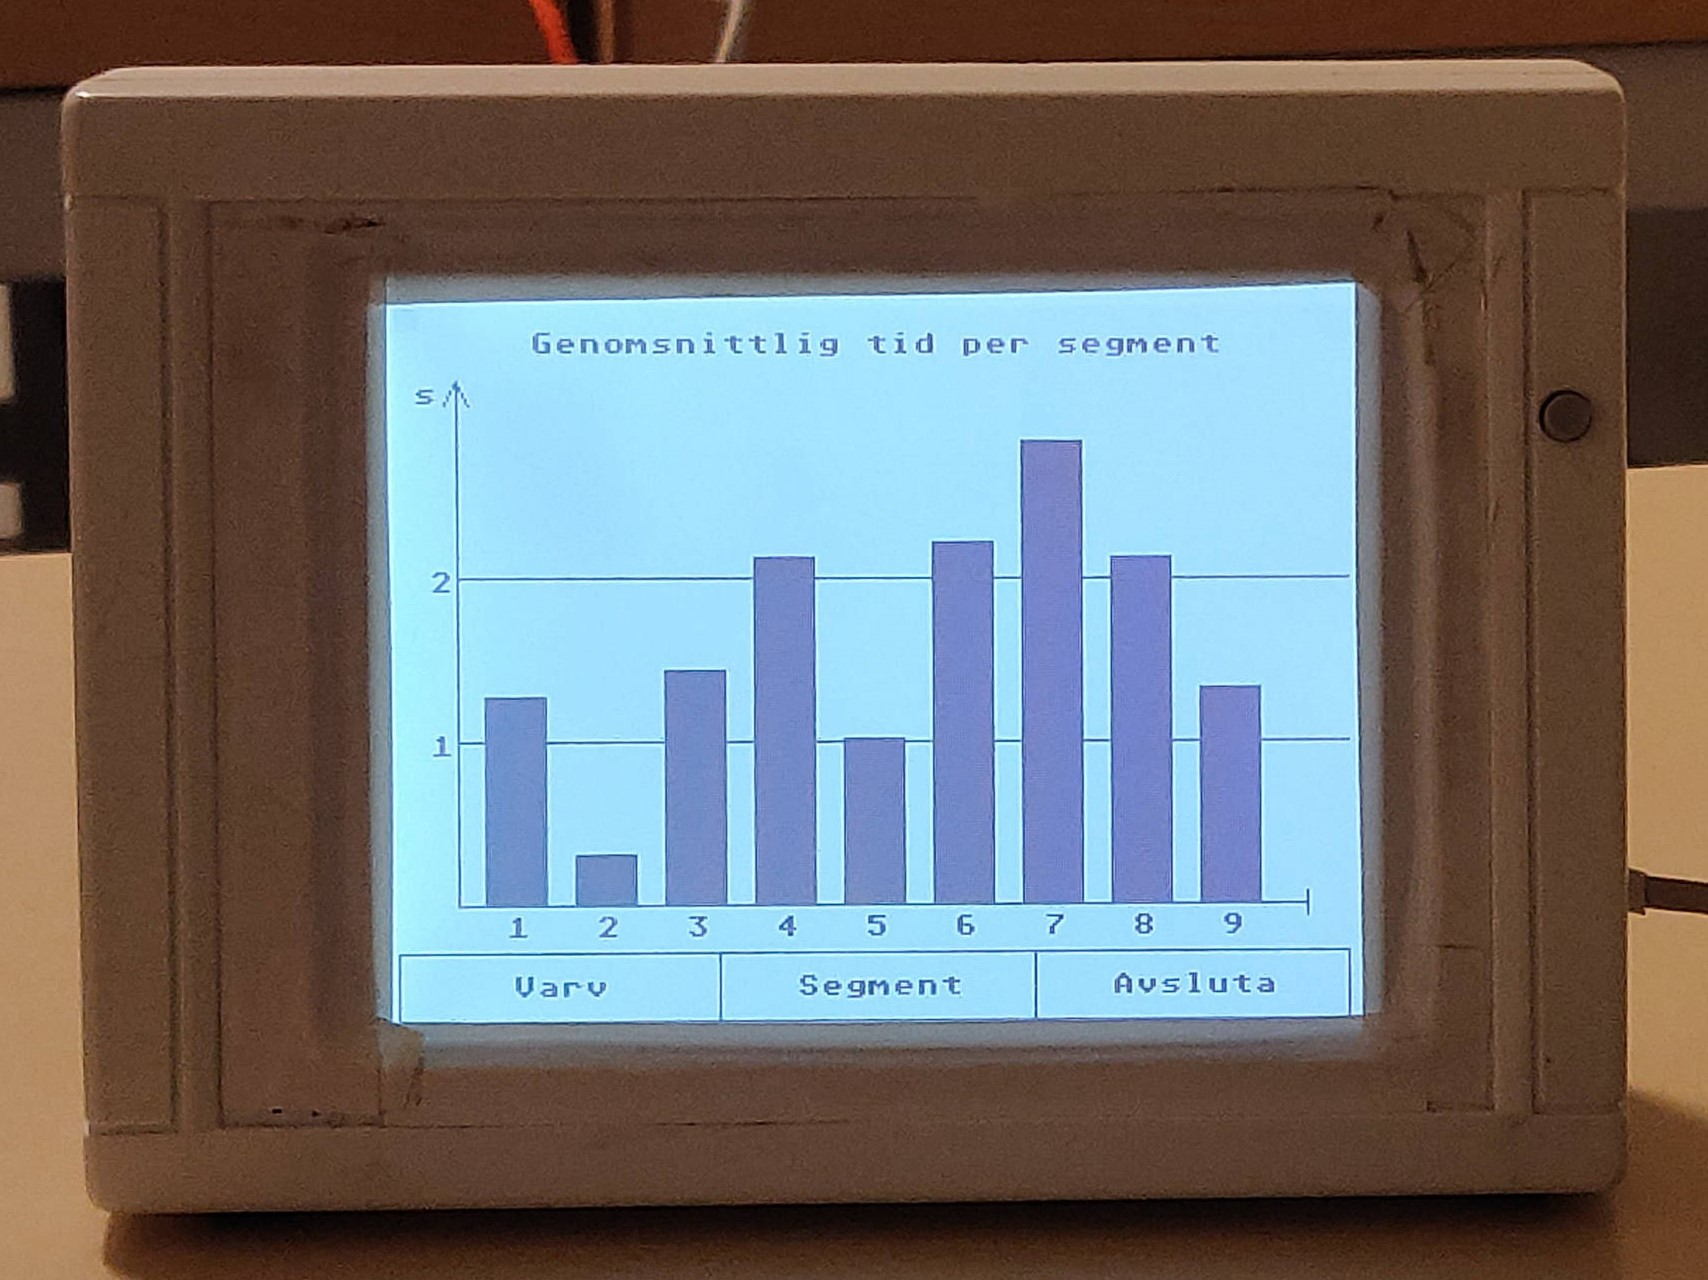
\includegraphics[width=0.75\linewidth] {Figures/genomsnitt_segment}
	\caption{Genomsnittliga segmentstider}
	\label{fig:display-seg}
	
	\vspace*{2\floatsep}% https://tex.stackexchange.com/q/26521/5764
	
	\centering
	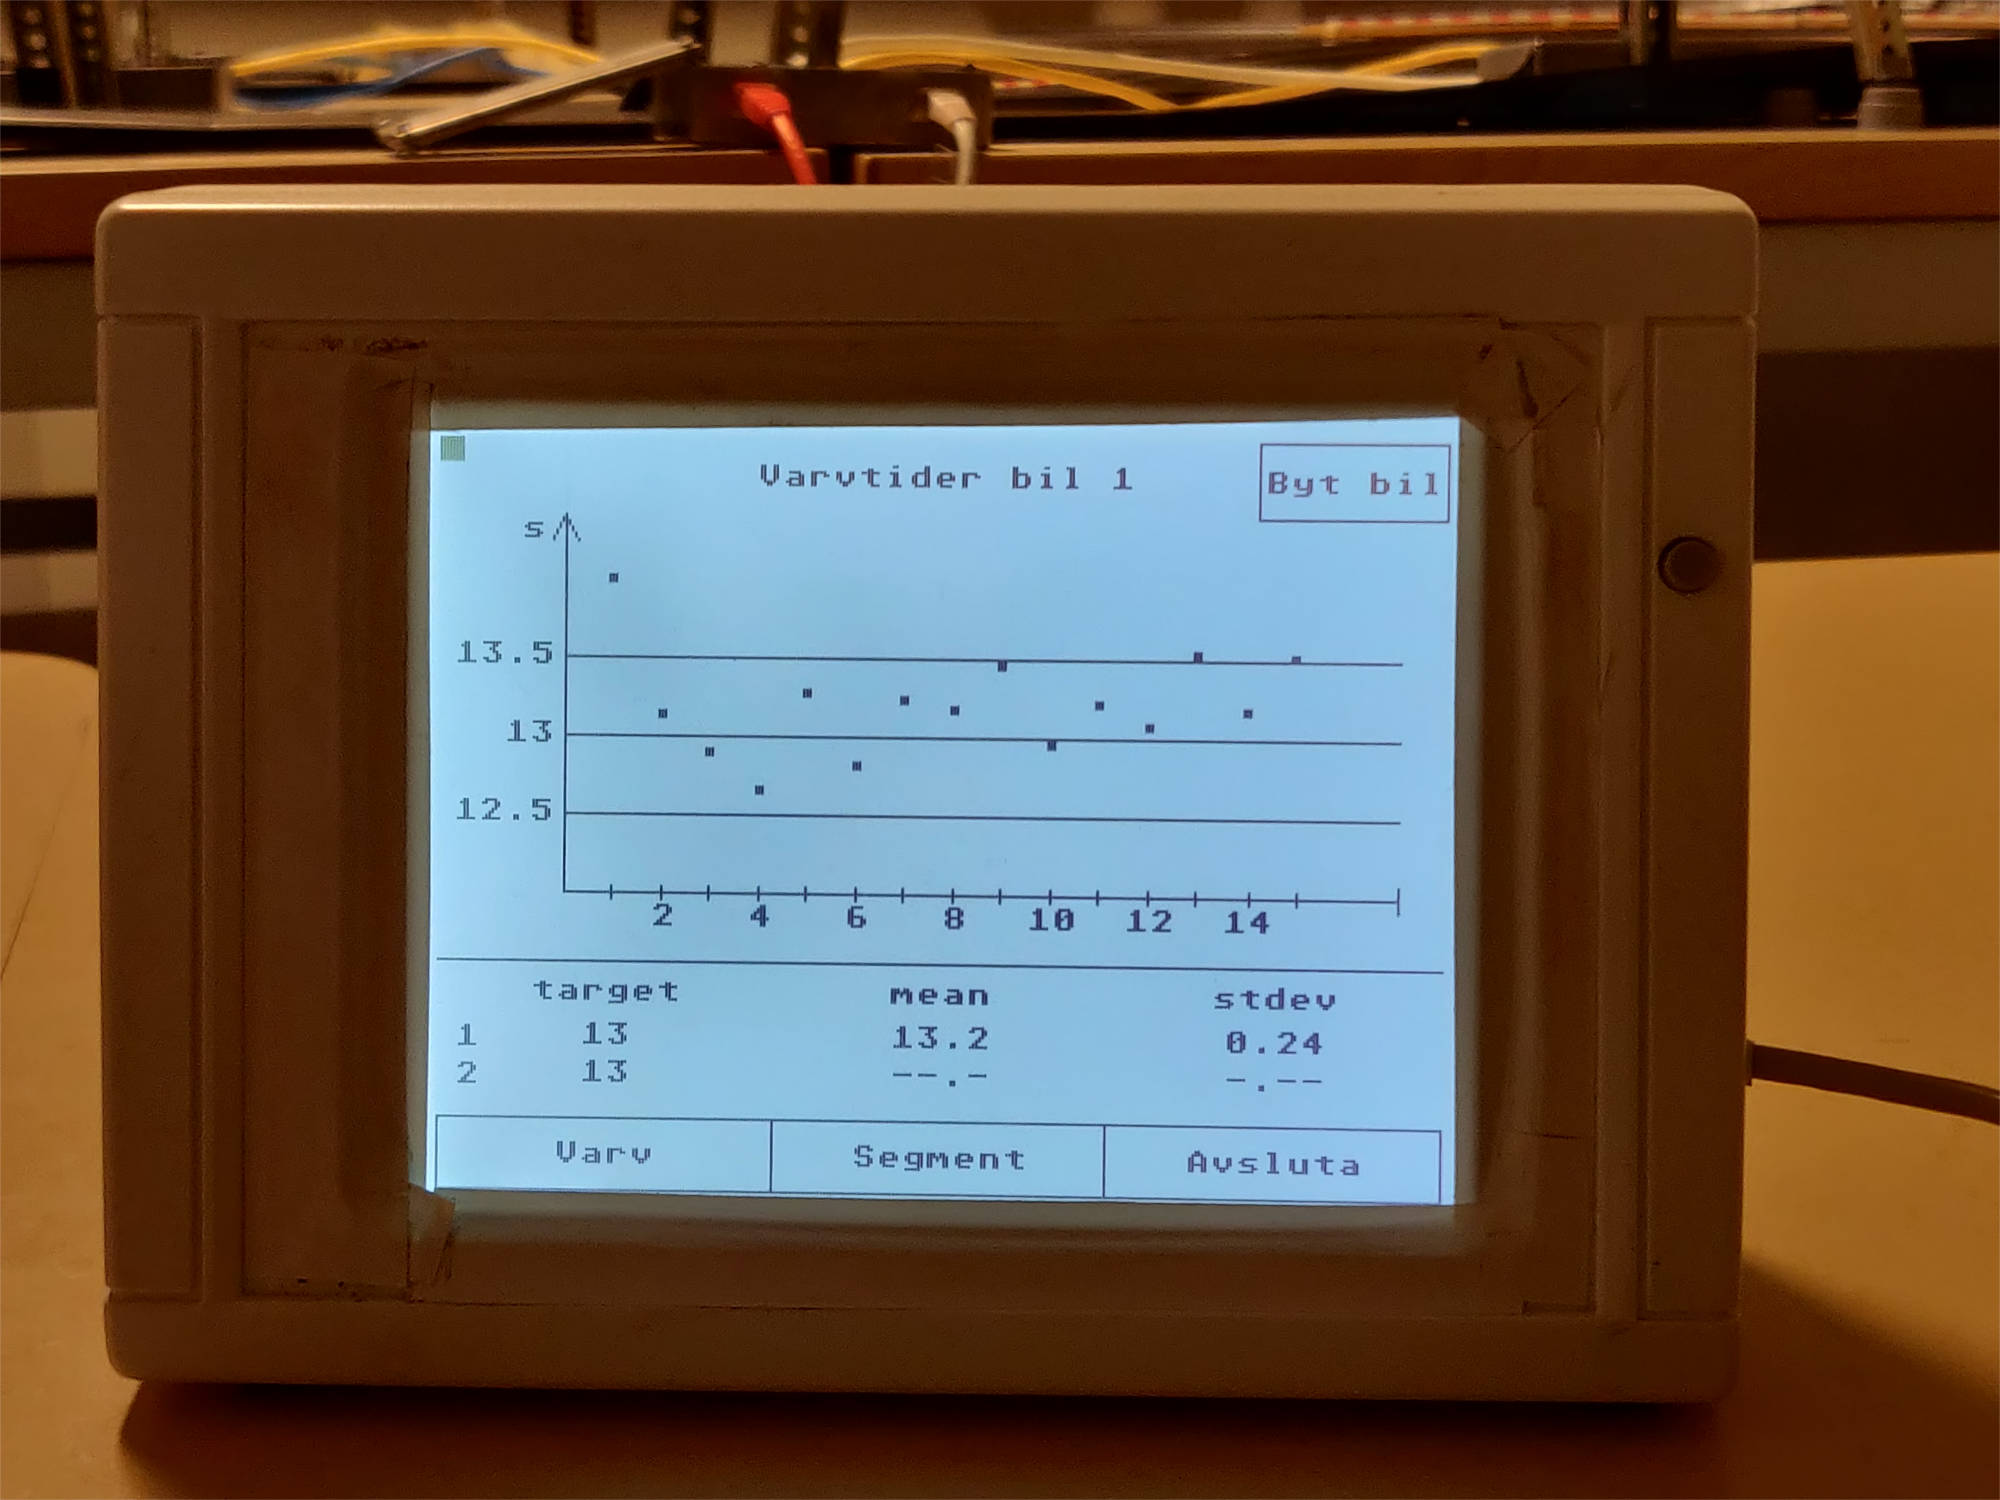
\includegraphics [width=0.75\linewidth] {Figures/varvtider}
	\caption{Varvtider}
	\label{fig:display-lap}
\end{figure}

\section{Resultat}

Vid redovisningstillfället slutfördes två körningar på 15 varv vardera där de
fem första var kalibreringsvarv (enligt krav 20 och 22). Vid den första
körningen var referenstiden inställd på 13 sekunder och vid den andra var
referenstiden inställd på 14 sekunder. De två körningarna finns uppritade i
Figur~\ref{fig:laptimes-calibration} med kalibreringsvarven och i Figur~
\ref{fig:laptimes-no-calibration} utan kalibreringsvarven med vald referenstid
och den maximalt tillåtna avvikelsen på 0,5 sekunder (enligt krav 21) inritat.
Figur~\ref{fig:segtimes} visar den genomsnittliga segmentstiden vid vardera
körning och Tabell~\ref{table:resultat} visar resultaten beskrivna nedan.

Vid den första körningen höll bilen en genomsnittlig varvtid på 13,22~sekunder
med en standardavvikelse på 0,24~sekunder. $\pm$0,5~sekunder överträddes vid två
av varven med varvtider på 13,54 och 13,52~sekunder. Vid den andra körningen höll bilen en genomsnittlig varvtid på 14,47~sekunder
med en standardavvikelse på 0,26~sekunder. $\pm$0,5~sekunder överträddes vid
fyra av varven med en maximal överträdelse på 0,31~sekunder långsammare än
maximal tillåten varvtid (14,5~sekunder).

Ingen av dessa körningar uppfyllde kraven på prestanda, alltså krav 20, 21 och
23. Givarna lästes av mer än 10 gånger per sekund under båda körningarna.
Se~\ref{sec:system:korning:cykel} för information om hur detta uppmätts.

\begin{figure}
	\centering
	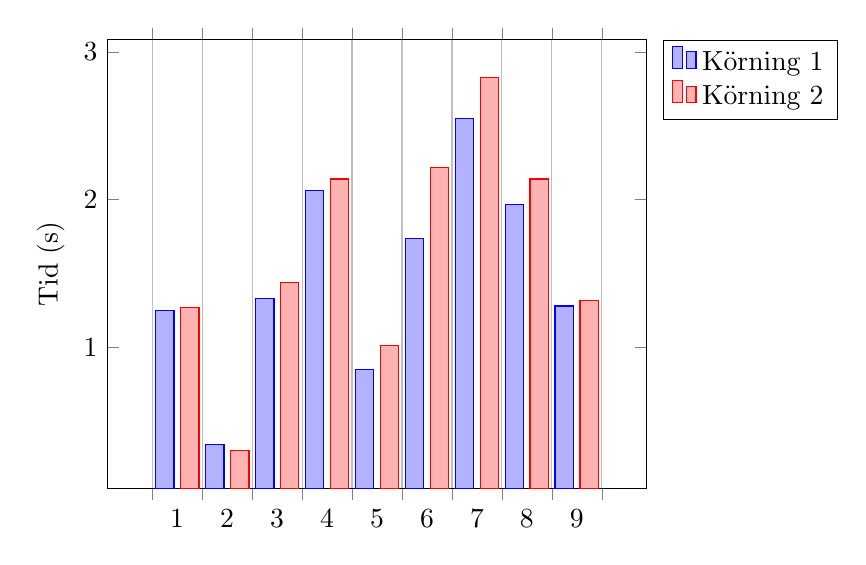
\begin{tikzpicture}
		\begin{axis} [
				ylabel=Tid (s),
				legend pos = outer north east,
				ybar interval=0.75
		]
			\addplot+ [] coordinates {(1, 1.25) (2, 0.34) (3, 1.33) (4, 2.06) (5, 0.85)
			(6, 1.74) (7, 2.55) (8, 1.97) (9, 1.28) (10, 1)};
			\addlegendentry{Körning 1}
			\addplot+ [] coordinates {(1, 1.27) (2, 0.30) (3, 1.44) (4, 2.14) (5, 1.01)
			(6, 2.22) (7, 2.83) (8, 2.14) (9, 1.32) (10, 1)};
			\addlegendentry{Körning 2}
		\end{axis}
	\end{tikzpicture}
	\caption{Genomsnittlig segmentstid för de två körningarna från redovisningen.}
	\label{fig:segtimes}
\end{figure}

\begin{table}
	\centering
	\caption{Resultaten från de två körningarna.}
	\begin{tabular}{|c|c|c|c|}
		\hline
		Körning & Referenstid & Snitt & Standardavvikelse \\\hline
		1 & 13 & 13,22 & 0,24 \\\hline
		2 & 14 & 14,47 & 0,26 \\\hline
	\end{tabular}
	\label{table:resultat}
\end{table}

\begin{figure}
	\centering

	\begin{tikzpicture}
		\begin{axis} [xmin=0, xmax=15.5,ymin=10,ymax=20, xlabel=Varv, ylabel={Tid (s)}, 
						legend pos=outer north east]
			\addplot+ [blue, mark options={blue}, mark=square*] table [col sep=comma, x index=0, y index = 1] {stats/lap.csv};
			\addlegendentry{Körning 1}
			\addplot+ [red, mark options={red}, mark=*] table [col sep=comma, x index=0, y index = 2] {stats/lap.csv};
			\addlegendentry{Körning 2}
		\end{axis}
	\end{tikzpicture}
  \caption{Varvtider för de två körningarna från redovisningen, inklusive
	kalibreringsvarven.}
	\label{fig:laptimes-calibration}

	\vspace*{\floatsep}% https://tex.stackexchange.com/q/26521/5764

	\begin{tikzpicture}
		\begin{axis} [xmin=5.5, xmax=15.5,ymin=12,ymax=16, xlabel=Varv, ylabel={Tid (s)}, 
						legend pos=outer north east]
			\addplot+ [blue, mark options={blue}, mark=square*] table [col sep=comma, x index=0, y index = 1] {stats/lap.csv};
			\addlegendentry{Körning 1}
			\addplot[blue, domain=0:20] {13};
			\addlegendentry{Referenstid körning 1}
			\addplot+ [red, mark options={red}, mark=*] table [col sep=comma, x index=0, y index = 2] {stats/lap.csv};
			\addlegendentry{Körning 2}
			\addplot [red, domain=0:20] {14};
			\addlegendentry{Referenstid körning 2}
			\draw[dotted] (axis cs:0,12.5) -- (axis cs:16,12.5);
			\draw[dotted] (axis cs:0,13.5) -- (axis cs:16,13.5);
			\draw[dotted] (axis cs:0,14.5) -- (axis cs:16,14.5);
		\end{axis}
	\end{tikzpicture}
	\caption{Varvtider för de två körningarna från redovisningen, exklusive
	kalibreringsvarven.}
	\label{fig:laptimes-no-calibration}
\end{figure}


\cleardoublepage
\appendix
\section{Handhavande}
Proceduren till handhavande för Matlab:

Starta Matlab 2015b. Observera att användaren måste använda datorn som finns
inne i bilbanerummet och som är inkopplade till bilbanan. Väl inne i Matlab
öppna filvägen för hårdisk X: och hitta sökvägen till yc4\_2019.

Därefter markera och högerklicka på mappen kod och där kommer ett alternativ som
heter Add To Path. Välj sedan Select Folders And Subfolders som dyker upp när
musen pekar på Add To Path. Därefter expandera bilbana mappen följt av yc4
mappen. Öppna sedan main.m och starta systemet genom att klicka på Run i Editorn
i Matlab.

När koden körs i Matlab är dags att starta bilarna detta görs genom att via den
externa touch displayen. Där finns möjligheterna att välja antalet banor som ska
köras samt möjligheten att justera referenstiden. Kryssa även i om någon av
banorna ska köras manuellt. Därefter starta genom att trycka på knappen nere i
det högra hörnet på displayen.

När programmet ska avslutas klickar användaren i kommentar fönstret i Matlab och
klickar på q om bilen ska stanna direkt. Om användaren istället vill att
bilen/bilarna ska stanna precis innan målgivaren klickar användaren på s
(observera att detta fungerar endast efter varv ett).

När programmet avslutas finns möjligheterna att se varvtiden/varvtiderna,
segmentstiden/segmentstiderna samt att avsluta. Detta väljs utifrån de tre
knapparna längst ner på displayen. Dessa knappar är Varv för att se varvtid,
Segment för att se segmentstider. Samt knappen Avsluta.

Om knappen Varv väljs kommer information såsom “target” vilket är vald varvtid.
“Mean” som är genomsnittlig varvtid och “Stdev” är standardavvikelsen. För att
se varvtiden för den andra banan klicka på knappen uppe i högra hörnet.

Om programmet kraschar: Om programmet kraschar öppna main.m. Därefter skriv in
ctrl och enter i avgränsningen som heter "\%\% END OF RACE" som finns i slutet av
koden main.m.

\section{Funktioner och filer}

\subsection{System}
\label{app:funktioner och filer:system}

\texttt{choose\_position(position, segment, track, track\_len)} - Körs när en
givare passerats. Gör en bedömning om en givare (eller flera) har missats genom
att kontrollera vilken givare som är närmast den nuvarande uppskattade position
och kompenserar om en givare bedöms ha missats. Se \ref{sec:missade givare}

\texttt{clamp(n, m, M)} - En hjälpfunktion som returnerar $n$ om $m < n < M$,
$m$ om $n < m$ och $M$ om $n > M$.

\texttt{detect\_missed(position, segment, track, track\_len)} - Returnerar true
om position ligger utanför det nuvarande segmentet.

\texttt{do\_boot(car, boot)} - Anropas en gång per programcykel i den så kallade
boostrap-fasen. Se \ref{sec:systembeskrivning:uppstart} för information.

\texttt{do\_car(car, t, displa\_data, boot)} - Anropas en gång per programcykel och innehåller ''Inhämtning av data'' och ''Behandling och sparande av data'' i figur \ref{fig:flow}.

\texttt{do\_gov(car)} - Anropas varje gång en givare passerats. Vid målgivaren
jämförs referenstiden och den förra varvtiden och car.constant anpassas efter
differensen mellan dem. Om differensen är högre ändras car.constant mer, och
vice versa om differensen är låg. Vid givare 5 och 8 jämförs referenstiden och
en uppskattning av hur lång tid det nuvarande varvet troligen kommer ta. Se
\ref{sec:systembeskrivning:governor} för mer information.

\texttt{fit\_percents(percents, lap\_time, seg\_times)} - Anropas vid varje nytt
varv. Räknar ut den procentuella tiden varje segment tog det förra varvet och
sparar medelvärdet mellan den förra procentsatsen och den nya, uträknade
procentsatsen. Procentsatsen normeras sedan så summan är 1 (100 procent).

\texttt{format\_seg\_times(car)} - Anropas när körningen avslutas. Returnerar
den genomsnittliga tiden för varje segment.

\texttt{get\_approx\_v(cur\_seg, car)} - Anropas varje programcykel. Uppskattar
bilens nuvarande hastighet genom att dividera den senast uppmätta segmentstiden
med segmentets längd.

% \texttt{get\_new\_u(new\_v, seg\_constant} - FLYTTA BERÄKNINGEN TILL DO\_CAR,
% BEHÖVER INTE VARA EN EGEN FUNKTION

\texttt{get\_new\_v(position, list)} - Anropas varje programcykel. Söker igenom
bankartan och returnerar värdet v som matchar position.

\texttt{get\_position(approx\_v, prev\_p, delta\_t)} - Anropas varje
programcykel. Räknar ut hur långt bilen rört sig sedan senaste programcykeln.

% \texttt{get\_seg\_constant(position, lap\_constants, track, track\_len)} - TA
% BORT

\texttt{get\_time\_as\_string(millis)} - Omvandlar en mängd millisekunder till
formatet ''mm:ss.s''. Till exempel omvandlas 1250 ms till "00:01.'' och 11240 till
"00:11.2".

\texttt{main.m} - Huvudskriptet som startar hela systemet. Det script som
programmet ligger i. I main.m ligger alla funktioner. Det är denna fil som ska
startas vid systemuppstart, se \ref{app:handhavande}

\subsection{Display}
\label{app:funktioner och filer:display}

\texttt{bar\_graph(direction, no, x1, x2, y1, y2, start\_value, end\_value,
type, pattern)} - Skapar ett stapeldiagram med ett hörn i \texttt{(x1, y1)} och ett
diagonellt hörn i \texttt{(x2, y2)}. \texttt{direction} är en av 'O', 'U', 'L' och 'R' och
bestämmer åt vilket håll "upp" är på stapeln. 'O' står för upp ('oben' på
tyska), 'U' står för ner ('unter'), 'L' står för vänster ('links') och 'R' står
för höger ('rechts'). Värdet stapeldiagrammet ska visa specifieras med
\texttt{update\_bar\_graph}. \texttt{start\_value} och \texttt{end\_value}
bestämmer vad som ska vara noll- respektive maxvärde för stapeldiagrammet.
\texttt{no} är stapeldiagrammets nummer och behöver specifieras när
stapeldiagrammets värde ska uppdateras. \texttt{type} sätts till 0 för en enkel stapel
och 1 för en stapel inuti en ram.

\texttt{clear\_display()} - Rensar displayen.

\texttt{continue\_line(x2, y2)} - Fortsätter en linje från den senast specifierade
linjens slut till \texttt{(x2, y2)}.

\texttt{draw\_line(x1, y1, x2, y2)} - Ritar en linje mellan \texttt{(x1, y1)} och
\texttt{(x2, y2)}.

\texttt{key(x1, y1, x2, y2, down\_code, up\_code, just, text)} - Skapar en
tryckbar knapp (till skillnad från en omkopplare, se \texttt{toggle()}) med
diagonella hörn i \texttt{(x1, y1)} och \texttt{(x1, y1)} och texten \texttt{text}. Hur
texten justeras beror på \texttt{just} där 'R' gör texten högerjusterad ('right'), 'C'
gör texten centerjusterad och 'L' gör texten vänsterjusterad ('left'). Om
knappen trycks ned läggs \texttt{down\_code} i displayens interna minne och om knappen
släpps läggs \texttt{up\_code} i displayens interna minne.

\texttt{point(x1, y1)} - Ritar en punkt i \texttt{(x1, y1)}. Punktens storlek kan
anpassas med \texttt{set\_point\_size}.

\texttt{put\_text(x, y, justification, text)} - Skriver texten \texttt{text} i
\texttt{(x, y)}. Hur texten justeras beror på \texttt{justification} där 'R' gör
texten högerjusterad ('right'), 'C' gör texten centerjusterad och 'L' gör texten
vänsterjusterad ('left'). Om \texttt{justification} är 'R' bestämmer \texttt{x}
och \texttt{x} textens övre högra koordinat, om \texttt{justification} är 'C'
bestämmer \texttt{x} och \texttt{x} textens mittre koordinat och om
\texttt{justification} är 'L' bestämmer \texttt{x} och \texttt{y} textens övre
vänstra koordinat.

set\_point\_size(n1, n2) - Sätter storleken på punkter och linjer som ritas ut.
\texttt{n1} är storleken i x-led (mellan 1 och 15 pixlar) och \texttt{n2} är
storleken i y-led (mellan 1 och 15 pixlar).

\texttt{toggle(x1, y1, x2, y2, down\_code, up\_code, just, text)} - Skapar en
tryckbar omkopplare (till skillnad från en knapp, se \texttt{key()}) med
diagonella hörn i \texttt{(x1, y1)} och \texttt{(x1, y1)} och texten
\texttt{text}. Hur texten justeras beror på *just* där 'R' gör texten
högerjusterad ('right'), 'C' gör texten centerjusterad och 'L' gör texten
vänsterjusterad ('left'). Om knappen aktiveras läggs \texttt{down\_code} i
displayens interna minne och om knappen avaktiveras läggs \texttt{up\_code} i
displayens interna minne.

\texttt{update\_bar\_graph(num, val)} - Skickar värdet \texttt{val} till
stapeldiagram *num*.

\section{Material}

Projektgruppen har av beställaren tillhandahållits en lokal med nedanstående
utrustning.

\begin{itemize}
	\item En strax under 20 meter lång bilbana med två banor, utrustad med givare som
		skickar en signal när en en bil passerar under dem.
	\item Två handkontroller för manuell körning av bilbanan.
	\item Två datorer, den ena inkopplad till banan som kan styra spänningen i de
		två banorna.
	\item Kod skriven i Matlab som kan styra vilken spänning som skickas till
		banan.
	\item En display med touchfunktionalitet (Electronic Assembly eDIP320J-8LWTP).
	\item Kod skriven i Matlab som kan tvåvägskommunicera med displayen.
	\item 13 bilar.
\end{itemize}

\input{appendix/04-tester}
\section{Kravbeskrivning}

Krav 1. Systemet är helt skrivet i matlab.

Krav 2. Systemet kan startas oavsett bil på banan.. 

Krav 3. Systemet klarar av att missa givare. 

Krav 4. När ett varv har körts så uppdaterar displayen vilket varv som nyss
genomfördes samt varvtiden. 

Krav 5. Under programmets gång visas det nuvarande gaspådraget. 

Krav 6. Efter att programmet avslutats visas information på displyen.

Krav 7. Systemet kan köras oavsett vilken bil som placeras på banan. 

Krav 8. Programmet hanterar driftsfall genom att kompensera en större eller
mindre styrsignal. 

Krav 9. Om systemet inte får en nt insignal i form av en passerad givare inom
tio sekunder pausas systemet och användaren får frågan om denne vill fortsätta
eller avsluta. 

Krav 10. Användaren har alternativet att köra en eller båda banorna samt hur
banorna ska köras, autonomnt eller manuellt. Det manuella alternativet uppfyller
inte krav 8 på beslut av beställaren. 

Krav 11. Kravet struket från beslut av beställare. 

Krav 12. Tillsammans med frågan om bana ett eller två ska köras frågar
programmet systemet om banan ska köras manuellt eller autonomt. 

Krav 13. För att starta programmet krävs att man kan öppna matlab och starta
programmet. Därefter kan användaren starta med hjälp av displayen.  
 
Krav 14. När systemet startar frågar programmet användaren vilka banor som skall
köras samt vilken referenstid de ska ha. 

Krav 15. Systemet ställer de frågor till användaren via touch displayen.

Krav 16. Enligt de två givna testerna åkte bilarna inte av banan.

Krav 17. När programmet startas frågar programmet användaren vilken referenstid
som ska strävas efter, detta görs i ett intervall ]12,15[ med justeringar på 0,5
sekunder upp eller ner. 

Krav 18. Enligt de två visade körningarna stannade inte bilarna under något
tillfälle. 

Krav 19. 

Krav 20. De två testkörningarna resulterade i en standardavvikelse på 0,22
respektive 0,24. Kravet är delvis uppnått. 

Krav 21. De två testkörningarna resulterade i att bilarna överskred gränsen på
0.5 ett fåtal gånger, kravet delvsi uppnått. 

Krav 22. Kraven var delvis uppfyllda efter 5 varv. 

Krav 23. Kravet struket av beställaren. 

Krav 24. Resultaten sparades och delades med beställaren via email.  

Krav 25. Efter avslutad körning visas statistik i form av de plottar som önskas
i kravspecifikationen. 

Krav 26. Efter avslutad körning sparas alla data i en fil.  

Krav 27. Längre upp i dokumentet beskrivs hur tidtagningen gick till och hur den
validerades.

Krav 28. 

Krav 29. Deltagande i projektet har angett den tid de jobbat efter varje moment. 

Krav 30. Handledaren har inte bidragit med hjälp i mer än 25h.

Krav 31. Efter att programmet avslutas visas den cykel som tog längst tid, då
den inte passerar 0,1 sekunder. 

Krav 32. Efter två veckor av projektet godkänndes projektplanen. 

Krav 33. Under projektvecka fyra godkändes designspecifikationen av beställaren. 

Krav 34. Under projektvecka fem redovisade projektgruppen kraven 2, 4, 31 samt 25. 

Krav 35. Under projektvecka sju redovisade projektgruppen kraven 3, 5, 10, 17
samt 18. Även de krav som uppfylldes under bp.4a visades. 

Krav 36. Under projektvecka nio redovisade projektgruppen samtliga Lrav som
uppfyllts tidigare samt alla krav i avsnitt 3.2.

Krav 37. Programvaran levererades under projektvecka 10. 

Krav 38. Den tekniska dokumentationen levererades under projektvecka 10. 

Krav 39. Under projektvecka tio hölls en slutleverans där gruppen visade upp
samtliga krav och höll en presentation över vad hur arbetet har sett ut. 

Krav 40. Inför varje beslutspunkt har önskade dokument varit beställaren
tillhandahållna innan 09:00 arbetsdagen innan mötet. 

Krav 41. Projektledaren har delat tidsrapportering samt eventuella
mötesprotokoll vid rätt tid de flesta av projektveckorna, kravet är därför
delvis uppnått.

Krav 42. Alla dokument samt all programvara har samlats i gitlab minst en gång i
veckan sedan projektvecka 2. 

Krav 43. Projektplan, designspecifikation, mötesprotokoll, teknisk
dokumentation, testprotokoll samt efterstudie har gjorts. 

Krav 44. Dokument samt programvaran har bearbetats samt lagrats på
http://gitlab.ida.liu.se/.  

Krav 45. Alla dokument framtagna av projektgruppen har levererats i pdf-format. 

Krav 46. Alla dokument skrivna av projektgruppen är är skrivet på formell
korrekt svenska.

Krav 47. Dokumentationen innehåller, 

Krav 48. Programmet är uppdelat i funktioner. 

Krav 49. Projektgruppen har samtlats på mint ett möte i veckan där alla
medlemmar har närvarat. Handledaren har inte närvarat vilket resulterar i ett
delvis uppnått krav. 


\end{document}

